\section{Two Paths of Approach}

\label{sec:two_modes}

The \DH{} cannot be reached as an object.
Its effects appear when a descriptive window is pushed toward
its limit.

Within generated spacetime,
this occurs through different observational windows.

\medskip
\begin{quote}
Spatial convergence and temporal convergence
are dual ways in which descriptive limits become visible.
\end{quote}
\medskip

\subsection{Spatial Convergence}

Approaching ever smaller scales leads into the quantum domain.

Particles lose classical localization,
fields fluctuate strongly,
and quantities such as position and momentum
cease to be simultaneously definable.

As the scale decreases further,
theory gradually loses stability.

Quantum fluctuations intensify,
and calculations develop divergences.

At the Planck scale,
the continuity of spacetime itself is expected to break down.

Distance and position lose meaning.

\medskip
\begin{quote}
Reducing scale exposes a local horizon-form.
\end{quote}
\medskip

This path is described by quantum theory and quantum field theory.
Divergence appears frequently,
and renormalization becomes indispensable.

\subsection{Temporal Convergence}

The second path arises through increasing velocity.

In relativity,
as velocity approaches the speed of light,
time dilation becomes extreme.

At the limit,
the required energy for a massive body diverges,
and the temporal structure of the frame is pushed to its boundary.

Simultaneously,
length contraction eliminates spatial extension
along the direction of motion.

\medskip
\begin{quote}
Approaching the speed of light exposes a temporal horizon-form.
\end{quote}
\medskip

This path is described by relativity.
Energy diverges toward infinity,
and a body with finite mass cannot reach the speed of light.
The structure of theory itself does not permit it.

\subsection{Unified Structure}

Though these two paths appear fundamentally different,
they share a common structural feature.

\medskip
\begin{quote}
Both paths lead to limits in the definability of spacetime structure.
\end{quote}
\medskip

In spatial convergence,
fluctuation destroys localization.

In temporal convergence,
extreme motion destroys temporal duration.

In both cases,
difference itself ceases to be well-defined.

\medskip
\begin{quote}
Different paths.\\
Related losses of definability.
\end{quote}
\medskip

This is not coincidence.

The problem of quantum gravity, viewed from this perspective,
is not simply a matter of integrating two theories.
It is a matter of understanding the structure
by which different observational windows expose related limits
of spacetime description.

\medskip
\begin{quote}
They are not different domains,
but different trajectories through related horizon-forms.
\end{quote}
\medskip

These approaches do not reveal an object beyond the boundary.
They reveal the recurrent condition
under which the structures that make physical description possible
begin to lose stability.

This structure is illustrated in Figure~\ref{fig:two_paths}.

\begin{figure}[htbp]
  \centering
  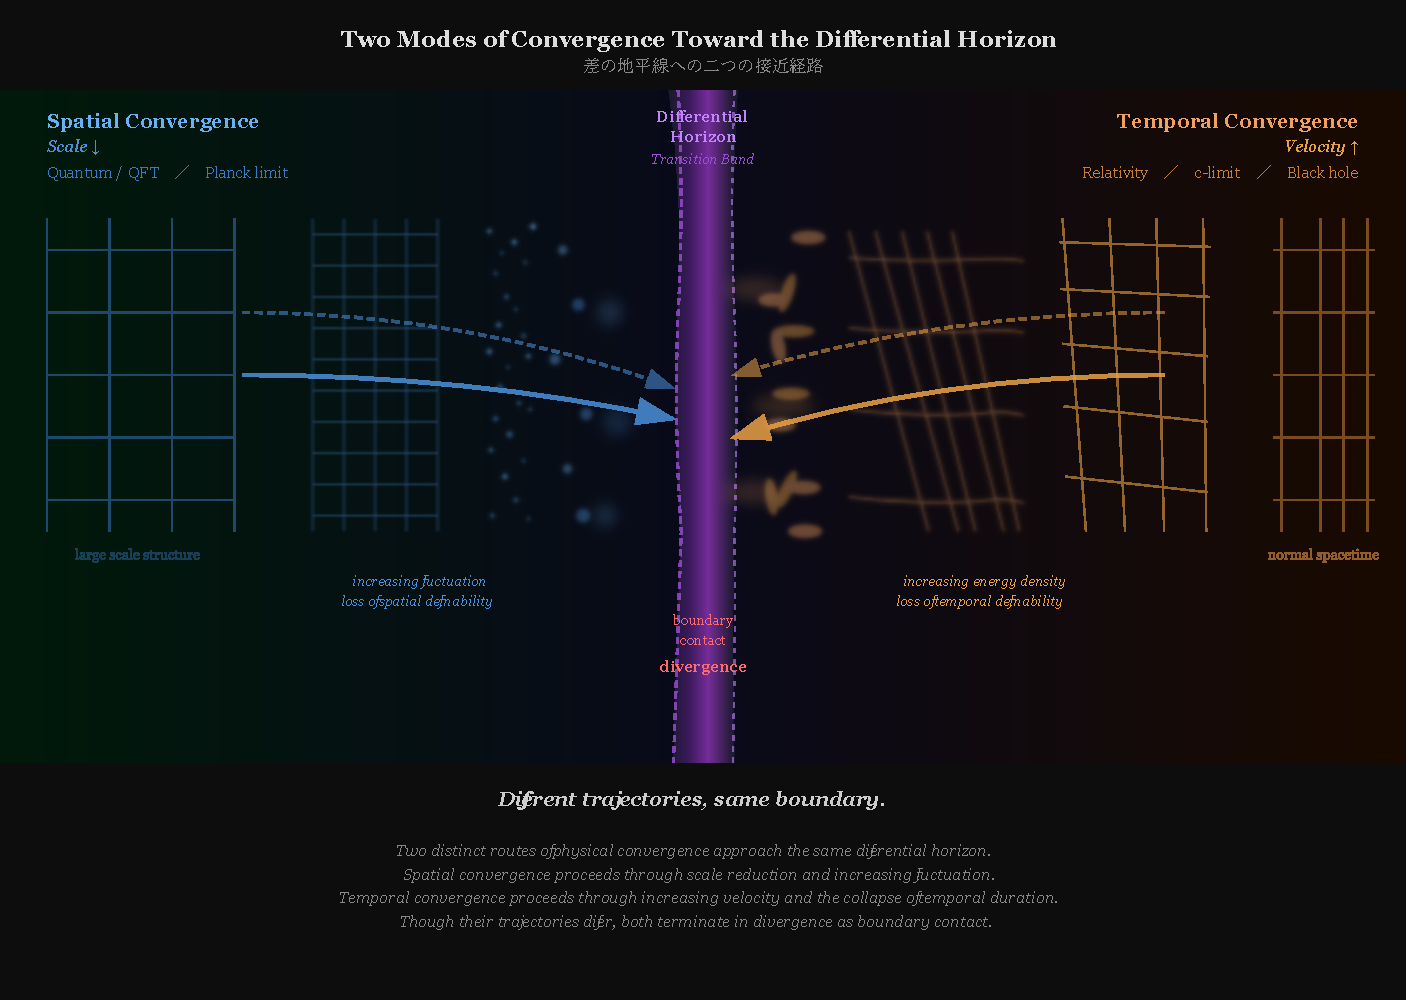
\includegraphics[width=\linewidth]{figures/figure2_two_convergences.pdf}
  \caption{%
    Two modes of convergence toward the \DH{}.
    Spatial convergence (left, blue) proceeds through scale reduction
    and increasing fluctuation toward the Planck limit.
    Temporal convergence (right, orange) proceeds through velocity increase
    and the collapse of temporal duration toward the speed-of-light limit.
    Both routes terminate in divergence as \bcontact{}.
    \textit{Different trajectories, related descriptive limits.}
  }
  \label{fig:two_paths}
\end{figure}

The next section redefines divergence formally
in light of this convergent structure.
